\documentclass{standalone}
\usepackage{tikz}
\usepackage{tkz-euclide}
\usepackage{ctex}
\pagestyle{empty}
\setCJKmainfont{Noto Serif CJK SC}
\usepackage{siunitx,chemmacros,chemfig}
\setchemfig{bond offset = 0pt}
\chemsetup[orbital]{
  overlay,
  opacity=0.5,
  sp/scale=2.5,
  s/color=blue!50,
  s/scale=1.8,
  p/scale=3.0
}
\begin{document}
\small
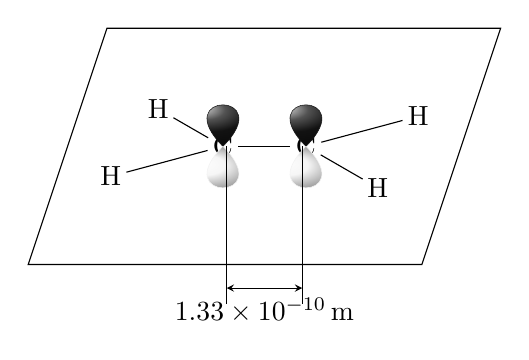
\begin{tikzpicture}[>=stealth]
  \draw(-3.0,-1.5)--(2.0,-1.5)--(3.0,1.5)--(-2.0,1.5)--cycle;
  \node {
  \chemfig{
    H-[:15,1.4]C({\orbital{p}})
    (-[:150,0.9]H)-C({\orbital{p}})
    (-[:15,1.4]H)
    (-[:-30]H)
    }
  };
  \draw[very thin](-0.48,0)--(-0.48,-2);
  \draw[very thin](0.48,0)--(0.48,-2);
  \draw[very thin,<->](-0.48,-1.8)--(0.48,-1.8)node[midway,below]{\qty{1.33e-10}{m}};
\end{tikzpicture}
\end{document}